%version of 04-02-19

\chapter{TECHNIQUES FOR ``DOING'' MATHEMATICS}
\label{ch:doingmath}

\begin{center}
{\it Entia non sunt multiplicanda praeter necessitatem.} \\
\hspace*{3in}{\footnotesize {\bf Occam's Razor}}
\end{center}

\noindent
This famous admonition by William of Occam (14th cent.) to strive for
simplicity is worth heeding when seeking mathematical models of
computational phenomena.

This is the chapter that ``amuses the palate''\footnote{\ldots in the
  sense of the French {\em amuse-bouche}.}~in preparation for the
introductory mathematical repast that we offer the reader.  Before we
present the hors d'oeuvres that we hope will entice the reader, we
``set the table'' for our feast.





Somewhat surprising to the non-mathematician, a large portion of
``doing'' mathematics, the widely touted ``queen of the
sciences''\footnote{See, e.g., Wolfgang Sartorius von Waltershausen,
  {\it Gauss zum Ged\"{a}chtniss} (1856).}, is {\em
  pattern-matching}---albeit of a monumentally sophisticated variety.
Mathematicians are trained to understand pieces of reality to a depth
that allows them to understand how apparently unrelated concepts $A$
and $B$ can be conceptualized via the same abstract representation,
and to analyze (computational, in our bailiwick) advantages to
exploiting such representations.  It may be useful to the reader to
keep the ``mathematics-as-pattern-matching'' metaphor in mind while
reading (from) this book, all the better to enjoy the many instances
of pattern-matching that populate its pages.

This chapter is devoted to the practice of mathematics within the
world of computing.  By means of plentiful examples, we hope to
convince the reader of the importance of mathematics in one's quest
for mastery over the technology and methodology of computing.  By
means of extensive explanations---we often prove the same fact many
times, from multiple, orthogonal vantage points, we hope to provide
the reader with tools for seeing the mathematical aspects of
computational settings and phenomena and technology and with
guidelines for using those tools effectively.

\section{Reasoning via Rigorous Proof}
\label{sec:reasoning-via-proofs}

Mathematics helps one thrive within the world of computing in two
ways: by enabling rigorous argumentation about properties of
computational structures and processes and by enabling cogent analyses
of such properties.  This section is devoted to the first of these
topics.  We survey, explain, and exemplify a range of proof techniques
tha are among most commonly useful within computational settings.

\subsection{Classical vs.~modern proofs and methodologies}
\label{sec:classical-v-modern-proofs}

Contrary to the all-too-common view of mathematics as arcane strings
of symbols that must be manipulated in rigid way, mathematics is a
vibrant, evolving system of thinking whose evolution is influenced by
the ever-changing objects that are being thought about and by the
ever-changing population that are doing the thinking.

Gone forever from the world of the practicing mathematician is the
rigidity that characterized the proofs and analyses of the 19th and
early-to-mid-20th century.
\begin{quote}
{\em We do not go back earlier than the 19th century because
formal notions of rigorous proof are, historically, a relatively
recent phenomenon, stemming largely from seminal philosophical
developments in the 19th century.}
\end{quote}
What has replaced the rigid logical systems and rigid prescribed forms
of ``antiquity'' is a vibrant system of thought that, when convenient,
\begin{itemize}
\item
represents the  number $n$, as convenient, by, e.g.,
  \begin{itemize}
  \item
a numeral in some positional number system, such as we use in daily
discourse,
  \item
a set (usually imagined) of $n$ balls or \ldots or widgets,
  \item
a unit-width rectangle that is $n$ units high.
  \end{itemize}

\item
freely uses different modes of argumentation (e.g., numerical and
structural induction, contradiction, counting, \ldots), even mixed and
matched throughout a single analysis;

\item
freely invokes a highly tested computer program to check mind-numbing
proliferations of clerically verifiable details.
\end{itemize}

Regrettably, mathematics education has lagged behind practice, despite
the emergence of technical/technological fields such as computer
science that cannot advance very far without at least informal
extensions and adaptations of the now-archaic formal proof systems.

The current volume is dedicated to trying to overcome people's
resistance to mathematical analysis and argumentation via a modernized
and humanized---but no less rigorous---methodology for ``thinking
mathematically'', especially within computational frameworks.  We
attempt to develop proof systems and methods that the reader can
comfortably develop facility with.

Our avenue for promoting mathematical {\em understanding} rather than
just rote knowledge abjures any specific formalism.  Instead, we
develop multiple proofs for the topics of discourse, involving
multiple representations of the objects being discussed and multiple
modes of argumentation.  The reader will be able to see a variety of
arguments for the same topic, which will hopefully enhance the
likelihood of discovering an approach that is congenial to each
reader's individual way of thinking.  By practicing proofs and
analyses regarding more and more topics, the reader will begin to find
it increasingly easy to state informally what ultimately needs to be
analyzed rigorously and to intuit how to embark on the path toward
such rigor.


\section{The Elements of Rigorous Reasoning}
\label{sec:elements-of-reasoning}

\subsection{Basic Reasoning}

{\em Distinguishing name from object}.
%
A fundamental stumbling block in the road to cogent reasoning arises
from the inability to distinguish names from the objects they denote.
A prime example within the world of computing resides in the inability
to distinguish a function (which can be viewed as an infinite set of
argument-value pairs) from a program, which can be viewed as a name
for the function.  {\bf Note} that the often-used view of a function
as a {\em rule} for assigning values to arguments should be avoided,
because it suggests -- \underline{\em erroneously} -- that an
implementable such rule always exists!

{\em Quantitative reasoning}.
%
Students should understand the foundational distinction between
``growing without bound'' and being innite.  Within this theme, they
should appreciate situations such as the following.  Every integer,
and every polynomial with integer coefficients, is finite, but there
are infinitely many integers and infinitely many polynomials.
Students should be able to verify (cogently but not necessarily via
any particular formalism) assertions such as the following.
\begin{itemize}
\item
Let us be given polynomials $p(x)$ of degree $a$ and $q(x)$ of degree
$b > a$, where $a, b$ need not be integers.  There must exist a
constant $X_{p,q}$ (i.e., a constant that depends on the properties of
polynomials $p$ and $q$) such that for all $x > X_{p,q}$, $p(x) <
q(x)$.

Thus, polynomials having bigger degrees eventually {\em
  majorize}---i.e., have larger values than---polynomials having
smaller degrees.

\item
Continuing with polynomial $q$ of degree $b$: For any real number $c >
1$, there exists a constant $Y_{c;q}$ (i.e., a constant that depends
on the properties of polynomial $q$ and constant $c$) such that for
all $x > Y_{c;q}$, $c^x > q(x)$.

Thus, exponential functions eventually {\em majorize} polynomials.
\end{itemize}

\subsubsection{The Elements of Formal Reasoning}

induction

proof by contradiction

\subsubsection{The Elements of Empirical Reasoning}

Empirical reasoning does not convey the certitude that formal
reasoning does.  




\subsection{What is a ``modern'' proof?}

We are interested in helping the reader learn intuitively compelling,
perspicacious techniques for proving interesting mathematical results.
But what exactly is a ``mathematical proof"---especially within the
context of computational systems and artifacts?  To answer this
question operationally, we follow the lead of the French mathematician
Ren\'e Thom, \index{Thom, Rene\'{e}} the Fields medal winning inventor
of catastrophe theory.  Thom famously defined a proof as an argument
that ``creates a corpus of evidence for educated readers that leads
to their adherence.''
\begin{quote}
{\em Est rigoureuse toute d\'{e}monstration, qui, chez tout lecteur
  suffisamment instruit et pr\'{e}par\'{e}, suscite un \'{e}tat
  d'\'{e}vidence qui entraine l'adh\'{e}sion.}
\end{quote}

% \textit{a rigorous process that creates a state of
%  evidence for educated readers who leads their adherence}.

%{\Denis Develop a simple example here? consider a graph and show that the sum of the degrees is equal to twice the number of edges.}

\subsubsection{A discussion of ``rigor''}

\subsubsection{Sample proofs}
\label{sec:sample-proofs}


\paragraph{\small\sf A. The average length of a carry in a binary counter}

\noindent {\it The problem.}
%
You add from $1$ to $n$, in increments of $1$ using a counter of
binary (or, base-$2$) numerals.  Each time you increment the counter,
there is a {\it carry}.  These carries have varying lengths; for
instance, when $n = 32 = 100000_2$, the carry-lengths range
from $0$---whenever you increment an even integer---to $5$---when you
increment $31 = 11111_2$ to achieve $32 = 100000_2$. \\
{\em Prove that the average carry as you go from $1$ to $n$ hs length $2$.}

\medskip

\noindent {\it The solution.}

\noindent
Half of the increments add $1$ to an even number, i.e., a number whose
binary numeral ends in ``$ \ldots 0$''.  These increments generate no
carry---or, equivalently, a carry of length $0$.

\noindent
One-quarter of the increments, which form half of the remaining
increments, execute a carry of length $1$, because they add $1$ to a
numeral that ends in ``$ \ldots 01$''.

\noindent
One-eighth of the increments, which form half of the remaining
increments, execute a carry of length $2$, because they add $1$ to a
numeral that ends in ``$ \ldots 011$''.

Continuing in this way, one can show that the average length of a
carry can be expressed in the form
\[ 
\frac{1}{2} \cdot 0 \ + \ \frac{1}{4} \cdot 1 \ + \ \frac{1}{8} \cdot
3 \ + \ \frac{1}{16} \cdot 4 \ + \ \cdots
\]
Using techniques that we cover in Chapter~\ref{ch:Summation}, one
verifies that this infinite series converges with the sum $2$.  \qed


\paragraph{\small\sf B. On meeting new people}

\noindent {\it The problem.}
%
You are attending a cocktail party that is populated by $n$ couples.
In order to create a warm atmosphere, the host requests that each
attendee shake the hand of every attendee that he or she does not
know.  \\
{\em Prove that some two attendees shake the same number of hands.}

\medskip

\noindent {\it The solution.}
%
This observation follows from the {\it pigeonhole principle}, which
states the following.

{\it If $n+1$ pigeons occupy $n$ pigeonholes, then some hole contains
  $2$ pigeons.}

\noindent
This principle guarantees that some two attendees shake the same
number of hands.  To wit, the number of people that each attendee {\em
  does not know} belongs to the set $\{ 0, 1, \ldots, 2n-2 \}$,
because each person knows him/herself and his/her partner.  Because
there are $2n$ handshakers (the pigeons) and $2n-1$ numbers of hands
to shake (the boxes), some two shakers must shake the same numbers of
hands.  \qed


{\Denis Should we add here the concept of Proof by computer?
Used for instance in the 4-color theorem...}





\subsection{Proof by (Finite) Induction}
\label{sec:Induction}

It is crucial that the reader appreciate the fact that proofs by
induction, such as we discuss in this section---and exemplify in
Section~\ref{sec:positive-integer-power}.C---are important tools for
{\em verifying} the correctness of alleged results, but induction by
itself is not a tool for {\em discovering} new results.


\subsubsection{The proof technique}


\subsubsection{Sample proofs: verifying summation formulas}
\label{sec:Proof-Induction}


We illustrate the proof technique of (Finite) Induction by proving the
correctness of two familiar summation formulas: (1) the sum of the
first $n$ positive integers and (2) the sum of the first $n$ odd
positive integers.

\begin{prop}
\label{thm:sum-1-to-n-induction1}
For all $n \in \N$,
\begin{eqnarray}
\nonumber
S_n \ \eqdef \ \sum_{i=1}^n \ i
 & \eqdef &
 1 + 2 + \cdots + (n-1) + n \\
\label{eq:sum-first-n1}
 & = & {1 \over 2} n (n+1) \\
\nonumber
 & = & {{n+1}  \choose 2}.
\end{eqnarray}
\end{prop}

\begin{proof}
For every positive integer $m$, let {\bf P}$(m)$ be the proposition
\[  1 + 2 + \cdot + m \ = \ {{m+1} \choose 2}. \]
Let us proceed according to the standard format of an inductive
argument.

{\bf 1.} Because ${\displaystyle {2 \choose 2}} = 1$, proposition {\bf
  P}$(1)$ is true.

{\bf 2.} Let us assume, for the sake of induction, that proposition
{\bf P}$(m)$ is true for all positive integers strictly smaller than
$n$.  In particular, then, {\bf P}$(n-1)$ is true.

{\bf 3.} Consider now the summation
\[ 1 + 2 + \cdots + (n-1) + n. \]
Because {\bf P}$(n-1)$ is true, we know that
\[ 1 + 2 + \cdots + (n-1) \ = \ {n \choose 2}.  \]
By direct calculation, we see that
\begin{eqnarray*}
{n \choose 2} + n
  & = & \frac{n(n-1)}{2}  \ + \ n \\ 
  & = & \frac{n^2 - n + 2n}{2} \\
  & = & \frac{n^2 + n}{2} \\
  & = & {{n+1} \choose 2}
\end{eqnarray*}

Because $n$ is an arbitrary positive integer, we conclude that
{\bf P}$(n)$ is true whenever
\begin{itemize}
\item
{\bf P}$(1)$ is true
\item
{\em and}
{\bf P}$(m)$ is true for all $m < n$.
\end{itemize}
By the Principle of (Finite) Induction, then, we conclude that {\bf
  P}$(n)$ is true for all $n \in \N^+$.
\qed
\end{proof}

\bigskip

We turn now to our second summation, which asserts that each perfect
square of a positive integer, say, $n^2$, is the sum of the first $n$
odd integers, $1, 3, 5, \ldots, 2n-1$.  This proof complements the
constructive proofs of the same result in
Proposition~\ref{thm:squares-odd-integers-Gauss}.

\begin{prop}
\label{thm:squares-odd-integers-induction1}
For all $n \in \N^+$,
\[
\sum_{k=1}^n \ (2k-1)
 \ = \ 1 + 3 + 5 + \cdots + (2n-1) \ = \ n^2.
\]
That, is, the $n$th perfect square is the sum of the first $n$ odd
integers.
\end{prop}

\noindent {\em Verification.}
%
For every positive integer $m$, let {\bf P}$(m)$ be the proposition
\[ m^2 \ = \ 1 + 3 + 5 + \cdots + 2m-1. \]
Let us proceed according to the standard format of an inductive
argument.

{\bf 1.} Because $1 \cdot 1 = 1$, proposition {\bf P}$(1)$ is true.

{\bf 2.} Let us assume, for the sake of induction, that proposition
{\bf P}$(m)$ is true for all positive integers strictly smaller than
$n$.  In particular, then, {\bf P}$(n-1)$ is true.

{\bf 3.} Consider now the summation
\[ 1 + 3 + 5 + \cdots + 2n-3 + 2n-1 \]
Because {\bf P}$(n-1)$ is true, we know that
\[ 1 + 3 + 5 + \cdots + 2n-3 + 2n-1 \ = \ (n-1)^2 + 2n-1.  \]
By direct calculation, we see that
\[ (n-1)^2 + 2n-1 \ = \ (n^2 -2n +1) + (2n-1) \ = \ n^2. \]
Because $n$ is an arbitrary positive integer, we conclude that
{\bf P}$(n)$ is true whenever
\begin{itemize}
\item
{\bf P}$(1)$ is true
\item
{\em and}
{\bf P}$(m)$ is true for all $m < n$.
\end{itemize}
By the Principle of (Finite) Induction, then, we conclude that {\bf
  P}$(n)$ is true for all $n \in \N^+$.
\qed



\subsubsection{Making guesses: the method of undetermined coefficients}
\label{sec:undetermined-coefficients1}
\index{method of undetermined coefficients}

Proofs by induction, as provided in
Section~\ref{sec:positive-integer-power}.C, are important tools for
{\em verifying} the correctness of alleged results, but induction by
itself is not a tool for {\em discovering} new results.  This section
is devoted to the {\em Method of Undetermined Coefficients}, a tool
that sometimes yields the ``guesses'' that can then be verified via
induction.  We illustrate the method by deriving a formula for the sum
of the first $n$ perfect squares.  Our derivation builds on prior
knowledge of two facts:
\begin{enumerate}
\item
A trivial proof by counting verifies that
\[ \sum_{k=0}^n \ k^0 \ = \ \sum_{k=1}^n \ 1 \ = \ n.  \]
\item
We know from Proposition~\ref{thm:sum-first-integers-Gauss} that
\[
\sum_{k=0}^n \ k^1 \ = \ \sum_{k=1}^n \ k \ = \ {1 \over 2}(n^2 + n)
\]
\end{enumerate}
\begin{quote}
It seems to be silly to include the case $n=0$ in our summations,
since that term does not affect the sum, but that case tells us that
the ``constant term'' in all of these polynomials---i.e., the
coefficient of $k^0$---is always $c_0 =0$.
\end{quote}

\begin{prop}
\label{thm:sum-of-squares}
For all $n \in \N$,
\begin{eqnarray}
\nonumber
S^{(2)}_n \ \eqdef \ \sum_{i=1}^n \ i^2 
 & \eqdef &
 1 + 4 + \cdots + (n-1)^2 + n^2 \\
\label{eq:sum-1-to-nsq1}
 & = & {1 \over 3} n^3 \ + \ {1 \over 2} n^2 \ + \ {1 \over 6} n
\end{eqnarray}
\end{prop}
\index{formula for the sum of the first $n$ squares}

The target quantity $S^{(2)}_n$ in the proposition is often expressed
in a more aesthetic form:
\[ S^{(2)}_n \ = \
{1 \over 6} n (n+1)(2n+1) \ = \
\frac{2n+1}{3} \cdot {n \choose 2}.
\]

\begin{proof}
Since summing $0$th powers thus gives us a degree-$1$ polynomial, and
summing $1$st powers gives us a degree-$2$ polynomial, it is not
unreasonable to guess that summing $2$nd powers would give us a
degree-$3$ polynomial.  This turns out to be a good guess!  To prove
this assertion, we must determine values for constants $c_1, c_2, c_3$
such that
\begin{equation}
\label{eq:symbolic-cubic1}
\sum_{i=0}^n \ k^2 \ = \ c_3 n^3 + c_2 n^2 + c_1 n.
\end{equation}
(Including the case $n=0$ leaves us with {\em three} constants to
determine rather than four: we know that the coefficient of $k^0$ is
$c_0 =0$.)

We begin our determination of the constants $c_1, c_2, c_3$ by
instantiating the symbolic polynomial in (\ref{eq:symbolic-cubic1}) at
the smallest three values of $n$.  Any three values will work; using
the {\em smallest} ones simplifies our calculations.  These
instantiations leaves us with the following system of linear
equations.  (The summations in (\ref{eq:undetermined}) indicate where
each linear equation in the system comes from.)
\begin{equation}
\label{eq:undetermined}
\begin{array}{lccccccccc}
1. &
{\displaystyle \sum_{i=0}^1 \ k^2}
   & = & c_3    & + & c_2   & + & c_1   & = & 1 \\
2. &
{\displaystyle \sum_{i=0}^2 \ k^2}
   & = & 8 c_3  & + & 4 c_2 & + & 2 c_1 & = & 5 \\
3. &
{\displaystyle \sum_{i=0}^3 \ k^2}
   & = & 27 c_3 & + & 9 c_2 & + & 3 c_1 & = & 14
\end{array}
\end{equation}

We use a form of the {\it Gaussian elimination}
algorithm\footnote{This algorithm is defined and validated in sources
  such as \cite{CLRS}.}~to solve the system by ``eliminating
variables.''  First, we rewrite equation 1 as
\[ 8 c_3 + 8 c_2 + 8 c_1 \ = \ 8 \]
and substract equation 2 from it, thereby obtaining the $2$-variable
equation
\begin{equation}
\label{eq:step1}
4c_2 + 6 c_1 \ = \ 3.
\end{equation}
We perform a similar calculation based on equations 1 and 3 in
system (\ref{eq:undetermined}):  We rewrite equation 1 as
\[ 27 c_3 + 27 c_2 + 27 c_1 \ = \ 27 \]
and substract equation 3 from it, thereby obtaining the $2$-variable
equation
\begin{equation}
\label{eq:step2}
18 c_2 + 24 c_1 \ = \ 13.
\end{equation}
We now rewrite equations (\ref{eq:step1}) and (\ref{eq:step2}) to
obtain the simplified system
\[
\begin{array}{ccccc}
72 c_2 & + & 108 c_1 & = & 54 \\
72 c_2 & + &  96 c_1 & = & 52
\end{array}
\]
We now see, via subtraction, that
\[ 12 c_1 \ = \ 2 \]
or, equivalently,
\begin{equation}
\label{eq:valueof-c1}
c_1 \ = \ 1/6.
\end{equation}

Now that we know the value of $c_1$, we can make the indicated
substitution and further simplify system (\ref{eq:undetermined}).
Since we now have only two variables, we can also eliminate any one
of the three equations in (\ref{eq:undetermined}).  We eliminate
equation 3 in the system in order to simplify our calculations from
this point on.  We now have the system
\begin{equation}
\label{eq:undetermined-step2}
\begin{array}{lccccc}
1. &
c_3  & + & c_2   & = & 5/6 \\
2. &
8c_3 & + & 4 c_2 & = & 14/3 
\end{array}
\end{equation}
We rewrite equation 1 in (\ref{eq:undetermined-step2}) as
\[ 8 c_3 + 8 c_2 \ = \ 20/3 \]
and subtract equation 2 from this version of equation 1.  We thereby
discover that
\[ 4 c_2 \ = \ 2, \]
or, equivalently,
\begin{equation}
\label{eq:valueof-c2}
c_2 \ = \ 1/2.
\end{equation}

Using the values we have discovered for $c_1$ and $c_2$, in equations
(\ref{eq:valueof-c1}) and (\ref{eq:valueof-c2}), respectively, we
finally use equation 1 of system (\ref{eq:undetermined}) to determine
the value of $c_3$:
\begin{equation}
\label{eq:valueof-c3}
c_3 \ = \ 1 - \ 1/2 \ - \ 1/6 \ = \ 1/3.
\end{equation}
We have, thus, derived equation~(\ref{eq:sum-1-to-nsq1}).

\medskip

The careful reader will note that we are not really done yet.  We
have derived our expression for $S^{(2)}_n$ under the as-yet
unjustified assumption that $S^{(2)}_n$ really is a cubic (i.e.,
degree-$3$) polynomial.  What we need now is an induction that will
verify our result.  With our previous illustrations as models, we
shall leave this final task to the reader.

%\noindent
%***************** \\
% Arny: IS THIS OK? \\
% Denis: YES
%***************** 
\qed
\end{proof}

With more (calculational) work, but no new (mathematical) ideas, one
can derive explicit expressions for the sum of the first $n$ $k$th
powers, i.e., the quantity $S^{(k)}_n$, for any positive integer $k$.


\subsection{Proof by Contradiction}
\label{sec:Contradiction}
\index{proof by contradiction}

\begin{quote}
{\em The importance of this proof technique has been recognized since
  antiquity, under the Latin names {\em contradictio in contrarium}
  and, perhaps less accurately, {\em reductio ad absurdum}.}
\end{quote}



\subsubsection{The Proof Technique}
\label{sec:contradiction-technique}
\index{proof by contradiction!technique}



The basic principle that underlies proof by contradiction is that the
following {\em metamathematical} assertions are logically equivalent.
\begin{itemize}
\item
Proposition $P$ {\sc implies} Proposition $Q$
\item
Proposition $\sim Q$ {\sc implies} Proposition $\sim P$
\end{itemize}

As with many of these {\em metamathematical} principles, there is a
corresponding {\em mathematical} equivalence, in this case,
Proposition~\ref{thm:contraposition}.
\[ [P \Rightarrow Q] \ \equiv \ [(\sim Q) \Rightarrow (\sim P)] \]


\subsubsection{Sample Proofs}
\label{sec:sample-contradictions}
\index{proof by contradiction!sample proofs}

\paragraph{\small\sf A. There are infinitely many primes}

The following result is traditionally attributed to the Greek
mathematician Euclid,
\index{Euclid}
one of the patriarchs of mathematics.

\begin{prop}
\label{thm:Primes-infinite}
There are infinitely many prime numbers.
\end{prop}

\begin{proof}
Let us assume, contrarily, that there are only finitely many primes.
Say, in particular, that the following $r$-element sequence enumerates
all (and only) primes, in order of magnitude:

$\mbox{\bf Prime-Numbers} \ = \ 
\langle P_1, \ P_2, \ \ldots, \ P_r \rangle$

\noindent where
\begin{itemize}
\item
$P_1 = 2$
\item
$P_2 = 3$
\item
$P_i < P_{i+1}$ for all $i \in \{1, 2, \ldots, r-1\}$.
\end{itemize}

We verify the {\em falseness} of the alleged completeness of the sequence
{\bf Prime-Numbers} by analyzing the positive integer
\[ n \ = \ 1 + \prod_{i=1}^r \ P_i \ = \ 1 \ + \ 
\left(P_1 \cdot P_2 \cdot \cdots \cdot P_r \right).
\]

We make three crucial observations.

\begin{enumerate}
\item
We note first that {\em the number $n$ is not divisible by any prime
number  in the sequence {\bf Prime-Numbers}.}

To see this, note that for each $P_k$ in the sequence,
\[
n / P_k \ = \ \frac{1}{P_k} \ + \ \prod_{i \neq k} \ P_i .
\]
Because $P_k \geq 2$, we see that $n / P_k$ obeys the inequalities
\[
\prod_{i \neq k} \ P_i \ < \ n/P_k \ < \ 1 + \prod_{i \neq k} \ P_i.
\] 
The discreteness of the set $\Z$---see
Section~\ref{sec:integers}.A---implies that $n / P_k$ is not an
integer, because it lies strictly between two adjacent integers.

\item
We note next that, because of assertion 1, if the sequence {\bf
  Prime-Numbers} actually contained {\em all} of the prime numbers,
then we would have to conclude that {\em the number $n$ is not
  divisible by any prime number.}

\item
Finally, we remark that the Fundamental Theorem of Arithmetic
(Theorem~\ref{thm:Fund-Thm-Arith}) implies that {\em every integer is
  divisible by (at least one) prime number}.
\end{enumerate}

We have a chain of assertions that lead to a mutual inconsistency: on
the one hand, the integer $n$ has no prime-integer divisor; on the
other hand, no integer can fail to have a prime-integer divisor!  Let
us analyze how we arrived at this uncomfortable place.
\begin{itemize}
\item
At the front end of this uncomfortable string of assertions we have
the assumption that there are only finitely many prime numbers.  We
have (as yet) no substantiation for this assertion.
\item
At the back end of this uncomfortable string of assertions we have
the ({\em rock solid}) Fundamental Theorem of Arithmetic
(Theorem~\ref{thm:Fund-Thm-Arith}).
\item
In between these two assertions we have a sequence of assertions, each
of which follows from its predecessors via irrefutable rules of
inference.
\end{itemize}
It follows that the {\em only} brick in this edifice that could be
faulty---i.e., the only assertion that could be false---is the
assumption that there are only finitely many prime numbers.  Since
this assumption leads to an inconsistent set of assertions, we must
conclude that the assumption is false!  We conclude from this
classical proof by contradiction that there are infinitely many prime
numbers.  \qed
\end{proof}



\subsection{Geometrical and graphical proofs}
\label{sec:unconventionalproofs}

\subsubsection{An old and simple example}

\subsubsection{Fubini's principle}
\label{sec:Fubini}

\cite{Fubini}
\index{Fubini, Guido}


\subsection{Proofs via the Pigeonhole Principle}
\label{sec:pigeonhole}

{\Denis Is it a technique by itself like the other ones or should it be integrated into another one -- on thus, which one?}

The proof technique we discuss now builds on an observation that is
almost embarrassingly obvious---yet its simplicity is exceeded by its
importance as a source of strikingly surprising results.

\subsubsection{The Proof Technique}

The technique, known variously as {\it the pigeonhole principle}
\index{pigeonhole principle}
or {\it Dirichlet's Box Principle}
\index{Dirichlet's Box Principle}
(after the French mathematician Peter Gustav Lejeune Dirichlet),
\index{Dirichlet, Peter Gustav Lejeune}
exploits the fact that if one has $n$ objects (say, pigeons) and $m <
n$ boxes (they're the pigeonholes), then any way of putting pigeons
into boxes must place at least two pigeons into the same box.


\subsubsection{Sample (Fun) Applications/Proofs}
\label{sec:pigeon-apps}


\paragraph{\small\sf A. Choosing a pair of matching socks} 

You have $n$ pairs of socks, the socks in each pair having a distinct
color (one pair of red socks, one pair of blue socks, \ldots).  Since
you wake up ``very slowly'', you want to grab some number of unpaired
socks that is certain to yield at least one pair of same-color socks.
Clearly, if you grab any $n+1$ socks (the pigeons), the pigeonhole
principle guarantees that you have at least one monochromatic pair,
because there are only $n$ distinct sock-colors (the boxes).


\paragraph{\small\sf B. Finding birthday-mates}

You are attending a conference and wander into a lecture that has 367
attendees (including you).  It is certain that at least two attendees
share the same birthday: there are 366 possible birthdays (the boxes
for a leap year) and 367 birthday-possessors (the pigeons).

{\Denis May be we can put this in exercice and add the anniversary paradox which state a similar question with probabilities?}


\paragraph{\small\sf D. Friends and strangers at a party}

We turn now to a somewhat more surprising result that can be proved
using the pigeonhole principle.  While we phrase the result in
anthropomorphic, ``homely'', terms, its formal statement identifies it
as a genre of ``unavoidable subgraph''
\index{unavoidable subgraph phenomena}
%
phenomenon within the theory of {\it graphs}.
\begin{quote}
Graphs are an immensely important mathematical construct that models
myriad situations that involve objects (possibly people) and
interrelationships between pairs of objects.
Chapter~\ref{Ch:Graphs-Trees} is devoted to studying graphs and the
situations they can be used to model---including the problem discussed
here.
\end{quote}
Here is the ``homely'' version of the {\it Friends and Strangers} problem.
\index{friends and strangers problem}

\begin{prop}
\label{thm:triangle-cotriangles}
In any gathering of six people, at least one of the following
assertions is true.

\noindent {\rm A.}
There is a group of three people who know each other.

\noindent {\rm B.}
There is a group of three people none of whom knows either of the
others.
\end{prop}

\begin{proof}
Let the gathering consist of six indistinguishable people, named
$P_1$, $P_2$, $P_3$, $P_4$, $P_5$, $P_6$.  Focus on an arbitrary
person, say $P_5$.  (This choice ``sounds'' more arbitrary than
$P_1$---but, of course, is not.)  Now, there are $5$ people, namely,
$P_1$, $P_2$, $P_3$, $P_4$, $P_6$, each of whom $P_5$ either {\em
  knows} or {\em doesn't know}.

Clearly, some $3$ of these $5$ people ``lie on the same side of the
{\em know/don't-know} fence.''  This follows from the pigeonhole
principle: we have {\em two} boxes ({\em know} and {\em doesn't know})
and {\em five} pigeons (the people $P_1$, $P_2$, $P_3$, $P_4$, $P_6$).
Any way of putting the pigeons into the boxes will place three people
into one of the boxes.

Say, with no loss of generality, that $P_5$ {\em knows} $P_1$, $P_2$,
$P_3$.
\begin{quote}\index{``with no loss of generality'': meaning}
Why can we claim that the selected situation--- ``$P_5$ {\em knows}
$P_1$, $P_2$, $P_3$''---can be assumed ``with no loss of generality''?
One should {\em always} ask this question about such a claim!  In the
current case, the claim follows from the following facts.

(a) The names that we use to refer to the six assembled people are
just for our expository benefit.  The names carry no inherent meaning
related to the {\it Friends and Strangers} problem.  You can repeat
our argument while choosing arbitrary replacements for $P_1$, $P_2$,
$P_3$, $P_5$, with no change to the logical outcome.

You can also interchange the {\em know} and {\em don't-know} labels.
The underlying logic will not change, although the conclusions
regarding options A and B in the statement of the proposition will
clearly ``flip''.
\end{quote}

Having decided that $P_5$ {\em knows} $P_1$, $P_2$, and $P_3$, we now
consider the implications of the possible relations between each of
the three pairs of people chosen from $\{P_1, P_2, P_3\}$.  There
are two logical possibilities.
\begin{itemize}
\item
Some two of $P_1$, $P_2$, $P_3$ know each other---say, with no loss of
generality, $P_1$ and $P_2$.  In this case, $P_1$, $P_2$, and $P_5$
form a trio of people who know one another (option A in the statement
of the proposition).
\item
No two of $P_1$, $P_2$, $P_3$ know each other.  In this case, $P_1$,
$P_2$, and $P_3$ form a trio of people none of whom knows either of
the others (option B in the statement of the proposition).
\end{itemize}
This disjunction completes the proof.

We close the proof by noting that nothing we have stated precludes the
possibility that {\em both} option A {\em and} option B are true!  \qed
\end{proof}


\section{Bijections between Sets and Combinatorial Proofs}

{\Denis A nice example but rather complicated here may be the proof of the little Fermat theorem}


\section{Reasoning via Mathematical Analysis}
\label{sec:analysis}

{\Denis I am not clear about this section.
What should it contain?}

%\subsection{Analyses via Linear Recurrences}
%\label{sec:linear-recurrences-1}
%
%\begin{theorem}[The Master Theorem for Linear Recurrences]
%\label{thm:master-thm-1}
%\index{The Master Theorem for Linear Recurrences}
%Let the function $F$ be specified by the following linear recurrence.
%\begin{equation}
%\label{eq:Lin-Recur:start-1}
%F(n) \ = \ \left\{
%\begin{array}{cl}
%a F(n/b) + c & \mbox{for } n \geq b \\
%c & \mbox{for } n < b
%\end{array}
%\right.
%\end{equation}
%Then the value of $F$ on any argument $n$ is given by
%\begin{equation}
%\label{eq:Lin-Recur:solve-1}
%\begin{array}{lclll}
%F(n) & = & (1 + \log_b n)c &  & \mbox{if } a=1 \\
%     &   &                 &  & \\
%     & = &
%  {\displaystyle
%  \frac{1-a^{\log_b n}}{1-a} \ \approx \ \frac{1}{1-a}
%  }
% &  & \mbox{if } a<1 \\
%    &   &                  & & \\
%    & = &
%  {\displaystyle
%\frac{a^{\log_b n} -1}{a-1}
%  }
% & & \mbox{if } a>1
%\end{array}
%\end{equation}
%\end{theorem}
%
%


\subsection{Asymptotics}
\label{sec:asymptotics}

{\em Asymptotics} can be viewed as a language and a system of
reasoning that allow one to talk in a {\em qualitative} voice about
{\em quantitative} topics.  We thereby generalize to arbitrary growth
functions terms such as ``linear'', ``quadratic'', ``exponential'',
and ``logarithmic''.

Such a language and system are indispensable if one needs to reason
about computational topics over a range of situations, such as a range
(``all existing''?)  computer architectures and software systems.  As
two simple examples: (1) Carry-ripple adders perform additions in time
linear in the lengths $n$ of the summands (measured in number of bits)
no matter what these lengths are. (2) Comparison-based sorting
algorithms can sort lists of $n$ keys in time proportional to $n \log
n$, but no faster---where the base of the logarithm depends on the
characteristics of the computing platform.  More precise versions of
the preceding statements require specication of the number $n$ and
other details, possibly down to the clock speeds of the host
computer's circuitry.

\subsubsection{The language of asymptotics}

The language of asymptotics, which has its origins in the field of
Number Theory in the late 19th century, builds on the following
terminology, which is likely what one would cover in an early
undergraduate course.  More advanced aspects of the language would
likely by beyond the needs of most students of computing, aside from
specialists in advanced courses.  The basics of the language build on
three primitive notations and notions.  Standard sources, such as any
text on algorithm design and analysis, flesh out the following ideas.
\begin{itemize}
\item
{\em The big-O notation}.
%
The assertion $f(x) = O(g(x))$ says, intuitively, that the function
$f$ grows no faster than function $g$.  It is, thus, the asymptotic
analogue of ``less than''.

Formally:
$f(x) = O(g(x))$

means

$(\exists c >0)(\exists x^{\#})(\forall x > x^{\#})
[f(x) \leq c \cdot g(x)]$

\item
{\em The big-$\Omega$ notation}.
%
The assertion $f(x) = \Omega(g(x))$ says, intuitively, that the
function $f$ grows at least as fast as function $g$.  It is, thus, the
asymptotic analogue of ``greater than''.

Formally:
$f(x) = \Omega(g(x))$

means

$(\exists c >0)(\exists x^{\#})(\forall x > x^{\#})
[f(x) \geq c \cdot  g(x)]$ \\

\item
{\em The big-$\Theta$ notation}.
%
The assertion $f(n) = \Theta(g(n))$ says, intuitively, that the
function $f$ grows at the same rate as does function $g$.  It is,
thus, the asymptotic analogue of ``equal to''.

Formally:
$f(x) = \Theta(g(x))$

means

$(\exists c_1 >0)(\exists c_2 >0)(\exists x^{\#})(\forall x > x^{\#})
[c_1 \cdot g(x) \leq f(x) \leq c_2 \cdot  g(x)]$
\end{itemize}
One renders the preceding intuitive explanations precise by pointing
out that the three specifies relations ($a$) take hold {\em
  eventually}, i.e., only for large arguments to the functions $f$ and
$g$, and ($b$) hold up to an unspecified constant of proportionality.

{\Denis I added a figure for illustrating the notations, do I have to change g and h in g1 and g2 in the figure?}
\begin{figure}[htb]
\begin{center}
       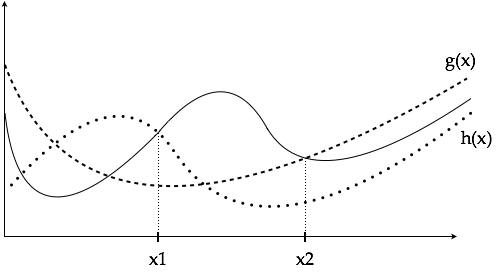
\includegraphics[scale=0.4]{FiguresArithmetic/NotationAsymptotic}
\caption{$g$ is a Big O of $f$ and $h$ is a Big Omega of $f$.}
\label{fig:Asymptotic}
\end{center}
\end{figure}

\ignore{*********
\subsubsection{Getting formal}

{\small\sf Big-$O$, Big-$\Omega$, and Big-$\Theta$ notation}.%
It is convenient to have terminology and a notation that allows us to
talk about the rate of growth of one function as measured by the rate
of growth of another.  We are interested in the exact growth rate, as
well as upper and lower bounds on the growth rate.  We do have
appropriate such language for certain rates of growth.  We can talk,
for instance, about a linear growth rate or a quadratic rate or an
exponential rate, to name just a few---and we get the desired bounds
using the prefixes ``sub'' or ``super,'' as in ``subexponential'' and
``superlinear''---but our repertoire of such terms is quite limited.
Mathematicians working in the theory of numbers in the late nineteenth
century established a notation that gives us an unlimited repertoire
of descriptors for growth rates, via what has come to be called the
big-$O$, big-$\Omega$, and big-$\Theta$ notations, which are
collectively sometimes called {\em asymptotic notation}.\index{asymptotic notation}
*******}

\subsubsection{The ``uncertainties'' in asymptotic relationships}

The formal definitions of all three of our asymptotic relationships
are bracketed by two important quantifiers:
\[ ``(\exists c >0)'' \ \ \ \mbox{ and } 
 ``(\forall x > x^{\#})''.
\]
The former, {\em uncertain-size} quantifier, asserts that asymptotic
notions describe functional behavior ``in the large''.  Thus, in
common with more common qualitative descriptors of quantitative growth
such as linear, quadratic, cubic, quartic, exponential, logarithmic,
etc., asymptotic relationships give no infomation about constants of
proportionality.  {\em We are not saying that constant factors do not
  matter!  We are, rather, saying that we want to discuss growth
  patterns \underline{in the large}.}

The latter, {\em uncertain-time} quantifier asserts that asymptotic
relationships between functions are promised to hold only
``eventually'', i.e., ``for sufficiently large values of the argument
$x$''.  Therefore, in particular, asymptotic notions cannot be
employed to discuss or analyze quantities that can never grow beyond a
fixed finite value.  The fact that all instances of a quantity
throughout history have been below $N$ is immaterial, as long as it is
conceivable that an instance larger than $N$ could appear at some time
in the future.

These quantifiers in particular distinguishes claims of asymptotic
relationship from the more familiar definite inequalities such as
``$f(x) \leq g(x)$'' or $f(x) \geq 7 \cdot g(x)$.  In fact, it is
often easier to think about our three asymptotic bounding assertions
as establishing {\em envelopes} for $f(x)$:
\begin{itemize}
\item
Say that $f(x) = O(g(x))$.  If one draws the graphs of the functions
$f(x)$ and $c \cdot g(x)$, then as one traces the graphs with
increasing values of $x$, one eventually reaches a point $x^{\#}$
beyond which the graph of $f(x)$ never enters the territory {\em
  above} the graph of $c \cdot g(x)$.
\item
Say that $f(x) = \Omega(g(x))$.  This situation is the up-down mirror
image of the preceding one: just replace the highlighted ``{\em
above}'' with ``{\em below}.''
\item
Say that $f(x) = \Theta(g(x))$.  We now have a two-sided envelope:
beyond $x^{\#}$, the graph of $f(x)$ never enters the territory {\em
  above} the graph of $c_1 \cdot g(x)$ and never enters the territory
{\em below} the graph of $c_2 \cdot g(x)$.
\end{itemize}
In addition to allowing one to make familiar growth-rate comparisons
such as ``$n^{14} = O(n^{15})$'' and ``$1.001^n = \Omega(n^{1000})$,''
we can now also make assertions such as ``$\sin x = \Theta(1)$,''
which are much clumsier to explain in words.

\medskip

\noindent {\bf Beyond the big letters.}
%
There are ``small''-letter analogues of the preceding ``big''-letter
asymptotic notations, but they are only rarely encountered in
discourse about real computations (although they do arise in the
analysis of algorithms).

\subsubsection{Inescapable complications}

The story we have told thus far is covered in many sources and
courses.  Two complications to the story are covered less faithfully,
although lacking them, one cannot perform cogent asymptotic
reasoning.  Both complications involve the notion of {\em uniformity}.

\noindent
{\bf 1.}
{\em Multiple functions}.
%
Say that we have four functions, $f, g, h, k$, and we know that both
\[ f(n) = O(g(n)) \ \ \mbox{ and } \ \ h(n) = O(k(n)) \]
It is intuitive that
\[ f(n) + h(n) = O(g(n) + k(n)) \]
--- but is it true?

In short, the answer is YES, but verifying that requires a bit of
subtlety, because, absent hitherto undisclosed information, the
proportionality constants $c_{f,g}$ and $N_{f,g}$ that witness the
big-$O$ relationship between functions $f$ and $g$ have no connection
with the constants, $c_{h,k}, N_{h,k}$ that witness the analogous
relationship between functions $h$ and $k$.  Therefore, in order to
verify the posited relationship between functions $f + h$ and $g + k$,
one much find witnessing constants $c_{f+h, g+k}$ and $N_{f+h,g+k}$.
Of course, this task requires only elementary reasoning and
manipulation --- but it must be done!

{\bf 2.}
{\em Multivariate functions}.
%
Finally, we discuss the scenario that almost automatically accompanies
the transition from a focus on sequential, single-agent computing to a
focus on PDC.  Within this broadened context, most functions that
describe a system have one or more variables that describe the
computing system --- its number of processors or of agents or the
sizes of its memory modules or the communication-radii of its
transponders or \ldots, in addition to the one or more variables that
describe the data that the system is processing.  Within such
scenarios, every assertion of an asymptotic relationship, of the form
\[ f(\vec{m}; \vec{n}) = O(g(\vec{m}; \vec{n})) \]
must explicitly specify the following information:
\begin{itemize}
\item
which variables can grow without bound;
\item
among such unbounded variables, which participate in the posited
asymptotic relation;
\item
for each participating unbounded variable $x$, what are the constants
$c_x$ and $N_x$ that witness the posited asymptotic relationship(s).
\end{itemize}

Clearly the complexity of cogent asymptotic reasoning --- hence also
the complexity of teaching about such reasoning --- gets much more
complicated in the multivariate settings engendered by PDC.  But, the
benefits of being able to reason qualitatively about the quantitative
aspects of computing increase at least commensurately!

\section{Coping with Infinity}
\label{sec:reasoning-infinity}

{\Denis is it the right place here?}

\subsection{Reasoning about Infinity}

{\Denis This part should be carefully read}

{\Arny An immediate problem is the forward reference to SUMMATION.  Do
  we need to reorganize?}

We presented in the chapter Summations several ways to compute the sum
of numbers in a given sequence ($a_n$).  If the sequence contains
infinitely many, the sum can be finite or not.  Some of the classical
techniques used while calculating finite sums are no longer valid for
infinite sums.


A natural definition is $\sum_{k \geq 1} a_k = lim_{n \rightarrow \infty} \sum_{k=1}^{n} a_k$.
But we have to be careful with this definition. 
For instance, let us consider the following paradoxal situation:
we aim to determine the value of $S = \sum_{k \geq 0} \frac{1}{2^k}$.
Defining the infinite sum as the limit leads to the value $2$. 
This is obtained $2S = S+2$...
But what happens if we apply the same reasoning to to the sum: $\sum _{k \geq 0} 2^k$?
Te obtain the value $-1$!
This is obviously not correct since the sum of increasing positive numbers should be positive.
The reason is that the terms of the series grows to $+\infty$.


\subsection{The ``Point at Infinity''}
\label{sec:point-at-infinity}

In large part, the difficulties encountered when dealing with infinite
objects result from the conceptual fiction that there is, in fact, a
``point at infinity''---i.e., that one can treat infinity as just
another number.  In many mathematical environments, this fiction is an
aid to reasoning which can be handled with totally rigor---but often
only when accompanied by rather sophisticated mathematical machinery.
Two familiar examples of such mathematical machinery are the notions
of \index{limit} {\it limit} and \index{continuity} {\it continuity}
(of a function).  A more advanced example of such machinery is the
{\it Riemann sphere}, \index{Riemann sphere} an invention of the
19th-century German mathematician Bernhard Riemann, \index{Riemann,
  Bernhard} which allows one to reason about the infinite
two-dimensional plane by ``conformally'' wrapping the plane into a
sphere whose ``south pole'' represents the zero-point (i.e., the
origin) of the plane and whose ``north pole'' represents the ``point
at infinity.''  There are many other, less-familiar, examples of such
mathematical machinery, including advanced topics such as {\it types}
in the domain of mathematical logic.

In the remainder of this text beyond the current section, we deal
successfully with a number of quite sophisticated topics related to
infinity.  To cite just two examples:
\begin{enumerate}
\item
In Chapter~\ref{ch:numbers-numerals} we successfully answer questions
such as
  \begin{enumerate}
  \item
{\it Are there more rational numbers than integers?}
  \item
{\it Are there more real numbers than rational numbers?}
  \end{enumerate}

\item
In Chapters~\ref{ch:numbers-numerals} and~\ref{ch:Summation}, we
successfully sum and manipulate infinite summations.
\end{enumerate}

The lessons of the preceding paragraphs is that there is no need to
avoid dealing with infinity and its related notions---as long as one
has the mathematical machinery necessary to define all needed notions
unambiguously, obtain well-defined results from all required
operations and manipulations, and reason cogently about all concepts
and processes.  That said, the scenarios described in the following
two subsections warn us to treat all aspects of infinity with care and
respect.  The subsections point out two challenges one can encounter
when reasoning about the infinite.  Both challenges leave us with a
{\em paradox}, i.e., ``a statement or proposition that, despite sound
(or apparently sound) reasoning from acceptable premises, leads to a
conclusion that seems senseless, logically unacceptable, or
self-contradictory.''  {\small (Apple dictionary)}


\subsubsection{Underspecified problems}
\label{sec:underspecified}

The paradoxes we present now require refined groundrules for their
resolution.  The underlying problems {\em seem} to be totally
specified---until one tries to develop their solutions.

\paragraph{\small\sf A. An infinite summation}

The first question we tackle was the subject of much concern as the
topic of infinite summations emerged from its infancy in the 18th
century.  The overriding question is, What can one learn from infinite
series that do not have a unique sum?  Much valuable work was done on
this question, most being beyond the scope of this text.  But the
conundrum presented by the following, particularly vexing, infinite
summation is valuable to consider here.
\[ S \ = \ 1 \ - \ 1 \ + \ 1 \ - \ 1 \ + 1 \ - \ 1 \ + \cdots \]
There are many conflicting, but well-reasoned, answers to the following
questions.

\noindent
{\bf Questions}:  {\it Does $S$ have a finite value?  If not, then is
  $S$ positive or negative?}

\noindent
Here are three plausible answers to these questions; the third merits
some strong contemplation.
\begin{enumerate}
\item
$S \ = \ 0$

This response is justified by the following association of terms in
the summation that defines $S$.
\begin{eqnarray*}
S & = & (1 \ - \ 1) \ + \ (1 \ - \ 1) \ + (1 \ - \ 1) \ + \cdots \\
  & = & 0 \ + \ 0 \ + 0 \ + \cdots \\
  & = & 0
\end{eqnarray*}

\item
$S \ = \ - \infty$

This response is justified by the following association of terms in the
summation that defines $S$.
\begin{eqnarray*}
S & = & 1 \ - \ (1 \ + \ 1) \ - \ (1 \ + \ 1) \ - \ (1 \ + \ 1)
          \ + \cdots \\
  & = & 1 \ - \ 2 \ - \ 2 \ - \ 2 \ - \cdots \\
  & = & - \infty
\end{eqnarray*}

\item
There is no valid answer, because the problem statement does not
specify how to associate terms.  Indeed, by mischievously playing with
parentheses, one can arrive at many ``plausible'' values for $S$.
This is one concrete example of how summations with infinitely many
terms behave differently from those with finitely nany terms.
\end{enumerate}


\paragraph{\small\sf B. The Ross-Littlewood paradox}

The following story about balls and bins is known as the {\it
  Ross-Littlewood paradox}, after its creators: A version of the story
appeared first in John Littlewood's enlightening and entertaining book
{\it Littlewood's Miscellany;} \cite{Littlewood-misc}
\index{Littlewood, John E.} the story was amplified to its present
form by S.M.~Ross \cite{Ross76}. \index{Ross, Sheldon M.}

Let us imagine a system that contains
\begin{itemize}
\item
a {\em really big} bin (in fact, one whose capacity grows as needed,
as the story progresses)
\item
an unbounded sequence of ordered balls, labelled 1, 2, \ldots
\item
a {\em very} (read: infinitely) precise clock.
\end{itemize}
The system is watched over by a {\it Keeper}.  We observe
the {\it Keeper} executing the following process.

Step $1$ of the process occurs at time {\em midnight minus $1$
  minute}.  The {\it Keeper} places the first ten balls in the
sequence (balls \#$1, \ldots, 10$) into the bin, and {\em immediately}
removes the first ball (ball \#$1$).

Step $2$ of the process occurs at time {\em midnight minus $1/2$
  minute}.  The {\it Keeper} places the next ten balls in the sequence
(balls \#$11, \ldots, 20$) into the bin, and {\em immediately} removes
the second ball (ball \#$2$).

The {\it Keeper} repeats this process endlessley, at midnight minus
$1/4$ minute (putting balls \#$21, \ldots, 30$ into the bin and
removing ball \#$3$), then at midnight minus $1/8$ minute (putting
balls \#$31, \ldots, 40$ into the bin and removing ball \#$4$), and
on, and on.

\noindent
{\bf Question}: {\it How many balls are present in the bin at
  midnight?}  (Note that ``infinity'' now measures the number of steps
executed in the process.)

\noindent
As in paragraph {\small\sf A}, there are many plausible answers to
this question.  We provide just three.
\begin{enumerate}
\item
There are infinitely many balls.

This response is justified by the following reasoning.  Each step of
the process inserts $10$ balls into the bin but removes only $1$ ball.
Hence, the population of the bin grows by $9$ balls after every step
of the process---and it never decreases!  Hence, the bin's population
after infinitely many steps must be infinite.

\item
There are $0$ balls---the bin is empty!.

This response is justified by the following reasoning.  Every ball is
eventually removed from the bin at some (finite) step of the process.
Specifically, ball \#$n$ is removed at step $n$, i.e., at time
midnight minus $2^{-n}$ seconds.

\item
There is no valid answer, because there is no ``moment at infinity''
that is encountered after an infinite number of steps of the process.
In other words, infinity is not a number!
\end{enumerate}


\paragraph{\small\sf C.  Zeno's paradox: Achilles and the tortoise}

In his celebrated {\it Paradox of Achilles and the Tortoise}, Zeno of
Elea \index{Zeno of Elea} \index{Zeno!Zeno's paradox} presented a
problem whose solution had to await the 17th century.  In the story,
the slow-footed Tortoise (T) tries to convince the speedy Achilles (A)
of the futility of trying to win any race in which A gives T even the
smallest head start.  As long as T is ahead of A, says T, every time A
traverses half the distance between himself and T, T will respond by
moving a bit further ahead.  Thereby, T will always be a positive
distance ahead of A, so that A can {\em never} catch T.  At first
glance, this story seems to call into question the physical reality of
all motion.

The resolution of the apparent paradox resides in the notion of
\index{infinitesimals} {\em infinitesimals}---quantities that
dynamically grow smaller than any finite number.  While familiar today
to anyone who has studied subjects such as the differential calculus,
the notion of infinitesimal actually dates back only a few hundred
years, to the 17th century.  Underlying the discovery/invention of
infinitesimals is one of the great real-life mysteries of all time:
Who invented/discovered infinitesimals.  The parties to this dispute
were the German mathematician Gottfried Leibniz \cite{Leibniz}
\index{Leibniz (Leibnitz), Gottfried Wilhelm} and the English polymath
(Sir) Isaac Newton \cite{Newton}.  \index{Newton, Isaac} The cases
favoring each of these great men contains enough merit to guarantee
that the dispute will likely never be settled.  We therefore list
Leibniz and Newton alphabetically and give a coarse dating of the 17th
century for the discovery.  This real-life mystery is as full of
intrigues and suspense as any that one encounters in fiction.


\paragraph{\small\sf D. Hilbert's hotel paradox}

While the final story of this section does not actually provide a
paradox, it does point out a fundamental difference between the real
world of finite capacities and an idealized world that is not so
encumbered.

Imagine that you are running a hotel that has an infinite number of
rooms which are labeled by the (entire set of) positive integers:
there is a room \#$1$, a room \#$2$, a room \#$3$, and so on.  Say
that on a particular evening, every room of the hotel is occupied by a
guest---and then a new guest arrives!

In a desire to accommodate the newcomer, you initiate the following
procedure, which was first proposed by the eminent German
mathematician David Hilbert. \index{Hilbert, David}

By means of a broadcast message to all current guests, you move each
guest who currently occupies room \#$k$ into room \#$k+1$.  Of course,
this total shift renders room \#$1$ available---so you assign this
room to the newly arrived guest.  The world is quiet once more!

Of course, this humorous story has its roots in a fundamental
distinction between the world of finite-capacity hotels that we live
in and the idealized infinite-capacity hotel proposed in Hilbert's
story.  In a word, every finite set of integers---think of the
integers as the room numbers in a finite-capacity hotel---{\em has a
  largest number}, while an infinite set of positive integers {\em
  does not have a largest number}.


\subsubsection{Foundational paradoxes}
\label{sec:paradoxes}

The ``foundational'' paradoxes that we present now can be resolved
only via the development of new, sophisticated, mathematical
machinery.

\paragraph{\small\sf A.  G\"{o}del's paradox: Self-referentiality in language}

Let us focus on the following utterance, which we call ``Sentence $S$''.

Sentence $S$: {\em The sentence you are reading at this moment is false.}

\noindent
{\bf Questions}: {\it Is Sentence $S$ true, or not?}

\noindent
Let us analyze the options.
\begin{itemize}
\item
On the one hand: \\
If Sentence $S$ is true, then one must accept its assertion that
Sentence $S$ is false.

\item
On the other hand: \\
If Sentence $S$ is false, then one must reject its assertion that
Sentence $S$ is false.  In other words, one must conclude that
Sentence $S$ is true.
\end{itemize}

\noindent
In the 1930s, the revolutionary philosopher/ logician Kurt G\"{o}del
\index{G\"{o}del, Kurt} turned the mathematical world on its head with
his demonstration that, roughly speaking,

\begin{tabular}{l}
{\em Any language that is self-referential---i.e., that can refer to
  its own sentences} \\
{\em as objects of discourse---must contain a sentence such as
  Sentence $S$, which} \\
{\em is neither true nor false.}  \cite{Goedel31}
\end{tabular}

The shocking implication of G\"{o}del's work is that in any
sufficiently sophisticated language $L$, the notions {\it true} and
{\it false} do not totally partition (into two pieces) the set of
legitimate utterances in language $L$.  The simplicity of Sentence $S$
and encodings thereof---see, e.g., \cite{Rosenberg09}---can be used to
show that the following classes of languages, and their kin, are
``sufficiently sophisticated'':
\begin{itemize}
\item
Natural languages (Swahili, German, Urdu, etc.)
\item
General-purpose programming languages (assembly language, Basic, C,
Java, LISP, Python etc.)
\item
Quantified mathematical languages---i.e., ones that contain logical
quantifiers such as {\sc for all} ($\forall$), {\sc there exist}
($\exists$), etc.
\end{itemize}

Of course, the world proceeded before G\"{o}del's earthshaking proof,
and it is still spinning after the proof.  We are just aware now that
we must be more careful in our use of language.  For instance, we must
employ pre-validated transformations in our compilers and
pre-justified ``small steps'' in our schedulers.


\paragraph{\small\sf B.  Russell's paradox: There is no ``anti-universal'' set}

The notion of set is perhaps the most primitive one in mathematics.
Even before delving into Chapter~\ref{ch:sets-BA-logic}'s survey of
the intricacies of sets and their mathematical kin, the reader
probably has at least an informal command of many of the relevant
notions.  One of the most basic features of sets is that their
elements are not governed by any {\it a priori} restrictions.  Most
specifically for our purposes here, a set can have sets as elements.
Indeed, there is no inherent reason why a set cannot contain itself as
an element!  At first blush, this possibility for self-membership
seems to be a rather innocuous freedom.  But, the 20th-century English
philosopher/logician Bertrand Russell
\index{Russell, Bertrand}
% and Alfred North Whitehead  \index{Whitehead, Alfred North}
pointed out in \cite{Russell02,Russell03} that, when encountered
within the world of potentially-infinite sets, the capacity for
self-membership is (intellectually) hazardous.

Russell had the foresight to observe that, absent any restrictions on
the formations of sets, one could talk about the following set $A$,
which we shall call ``anti-universal.''

{\em $A$ is the set of precisely those sets that {\em do not} contain themselves
  (as elements).}

\noindent
{\bf Question}.  {\it Is the set $A$ a member of itself?}

\noindent
Let us consider the possibilities.
\begin{itemize}
\item
If set $A$ is a member of itself, then by definition, $A$ {\em does
  not} contain itself---since sets belonging to $A$ {\em do not}
contain themselves.

\item
If set $A$ is not a member of itself, then by definition, $A$ is an
element of $A$.
\end{itemize}

There have been many attempts to reseolve the dilemma inherent in the
preceding analysis.  Many have striven for logical edifices that
declare the question ``{\it Is the set $A$ a member of itself?}''
somehow illegitimate.  One options that appeals to many is to assign
each sentence within a language $L$ a {\it type} (say, a positive
integer).  One then allows a sentence of $L$ to refer only to
sentences of lower type-number.

The strategem of typing utterances within a language $L$ disables
self-reference within $L$, hence defines away both Russel's paradox
and G\"{o}del's paradox.



